\chapter{Results}

\section{Local Training} \label{sec:local-training-results}

Die Ergebnisse der lokalen Trainingsdurchläufe sind wie zu erwarten etwas besser als im Federated Learning, auch wenn sie nicht der state-of-the-art entsprechen. Das liegt an dem einfachen und kleinen Modell, das ich für das Training genutzt habe.

Bei MNIST und SVHN erreicht das Modell bereits innerhalb von 10 Epochen gute Ergebnisse. Bei CIFAR-100 sind die Ergebnisse deutlich schlechter, weshalb ich hier mit einem \texttt{EarlyStopping}-callback gearbeitet habe. Trotzdem liegt die erreichte Accuracy unter 50\% (siehe \autoref{tab:local-model-results}).

\begin{table}
	\centering
	\begin{tabular}{|c|c|c|}
		\hline
		Dataset & Accuracy & Loss \\
		\hline
		MNIST & 0.9873 & 0.0382 \\
		SVHN & 0.8550 & 0.5106 \\
		CIFAR-100 & 0.4745 & 1.6995 \\
		\hline
	\end{tabular}
	\caption{The results of non-federated training without differential privacy}
	\label{tab:local-model-results}
\end{table}

Allerdings liegt der Fokus meiner Arbeit auf dem Federated Learning Algorithmus und die lokalen Trainingsdurchläufe sollten vor allem zum Vergleich und zum Finden von angemessenen Modellen und Hyperparametern dienen. Dafür war es hilfreich, denn ich konnte beispielsweise ein Feed-Forward Netz mit dem Convolutional Neural Network vergleichen. 

Die Trainingszeit liegt darüber hinaus ohne bei wenigen Sekunden oder Minuten. Derartige Experimente wären im Federated Learning sehr viel umständlicher gewesen, da es einen deutlich erhöhten Rechenaufwand mit sich bringt und auch deutlich instabiler ist was die Kovergenz der Modelle betrifft.

\begin{figure}
	\centering
	\begin{subfigure}{0.3\textwidth}
		\centering
		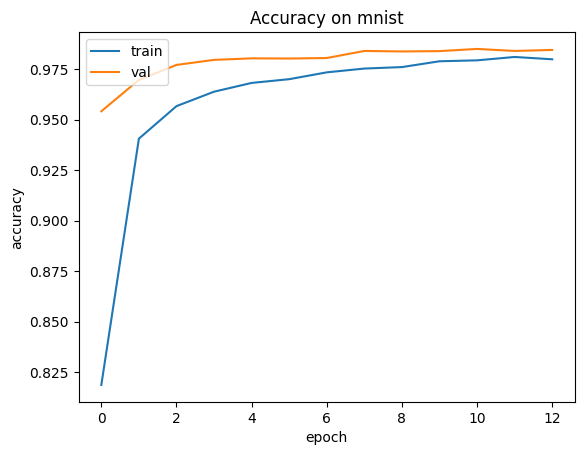
\includegraphics[width=\textwidth]{Bilder/mnist-results-local.png}
		\caption{}
	\end{subfigure}
	\begin{subfigure}{0.3\textwidth}
		\centering
		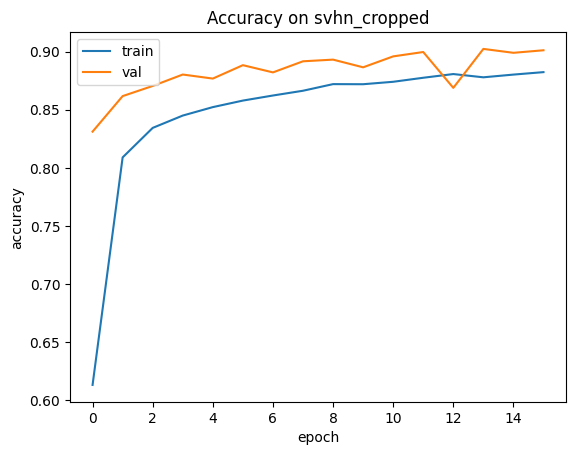
\includegraphics[width=\textwidth]{Bilder/svhn-results-local.png}
		\caption{}
	\end{subfigure}
	\begin{subfigure}{0.3\textwidth}
		\centering
		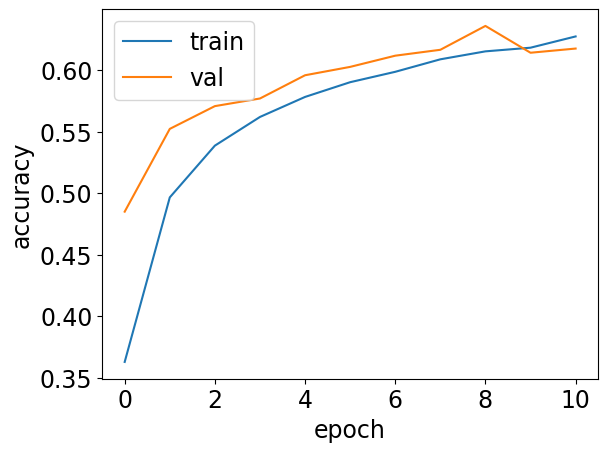
\includegraphics[width=\textwidth]{Bilder/cifar-results-local.png}
		\caption{}
	\end{subfigure}
	\label{fig:local-training-histories}
	\caption{Training and validation accuracies of the non-federated training processes}
\end{figure}

\section{Federated Training}

\subsection{MNIST}

Die Ergebnisse auf dem MNIST-Datensatz sind vielversprechend. Die Genauigkeit des Modells, das ohne Differential Privacy trainiert wurde, liegt nur knapp unter dem lokal trainierten Modell, was zeigt, dass das Federated Training auf dem Datensatz gut funktioniert.

Wie erwartet wirkt sich die Anwendung von Differential Privacy auf die Ergebnisse aus. Bereits die Anwendung des größten Privacy Budgets (\texttt{relaxed}) verringert die Genauigkeit deutlich.

Allerdings zeigt sich auch, dass die Anwendung von individualisierten Privacy Budgets hier deutlich besser funktioniert, als der allgemeine Ansatz, der das kleinste Budget auf alle Clients anwenden würde (\texttt{strict}).

Innerhalb der individualisierten Privacy Setups ist kaum ein Unterschied. In \autoref{fig:federated-mnist-results} schneidet \texttt{individual-strict} am Ende des Trainings sogar leicht besser ab als \texttt{individual-relaxed}, allerdings erreicht \texttt{individual-relaxed} bereits früher im Verlauf des Trainings bessere Werte. Allerdings sind die Unterschiede hier sehr gering.

\begin{figure}
	\centering
	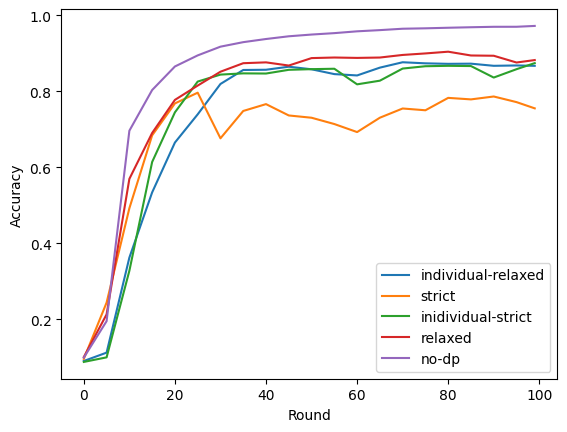
\includegraphics[width=0.7\textwidth]{Bilder/mnist-results.png}
	\caption{Accuracies of the different privacy setups during training on the MNIST dataset}
	\label{fig:federated-mnist-results}
\end{figure}

\begin{table}
	\centering
	\begin{tabular}{|c|c|c|}
		\hline
		Privacy Setup & Noise Multiplier & Accuracy \\
		\hline
		no-dp & 0.0 & 0.9721 \\
		relaxed & 0.9292 & 0.9042 \\
		individual-relaxed & 1.1368 & 0.8764 \\
		individual-strict & 1.2558 & 0.8741 \\
		strict & 1.5719 & 0.7963 \\
		\hline
	\end{tabular}
	\caption{The noise multipliers and the accuracies of the different privacy setups on the MNIST dataset}
	\label{tab:federated-mnist-noise-multiplier}
\end{table}

\subsection{SVHN}

\subsection{CIFAR-100}